\addtocontents{toc}{\protect\setcounter{tocdepth}{1}}
%La ligne ci dessus permet de masquer les subsections de l'intro dans la ToC

\section{Introduction}

\subsection{La Cryptographie}

\begin{frame}
\frametitle{Introduction}
    \begin{tikzpicture}[pin distance=1cm,every pin/.append style={font=\sffamily\itshape}]
    \node[alice,minimum size=2cm,pin={[text width=2em]40:{enc}}] (A) at (2,2) {Alice};
    \node[bob,mirrored, minimum size=2cm,pin={[text width=2em]140:{dec}}] (B) at (10,2) {Bob};
    \node[criminal,female,minimum size=2cm] at (6,-0.5) {Eve};
    \draw [thick,->] (A) -- (B) node[midway,above] {Message secret};
    \end{tikzpicture}
\end{frame}

\begin{frame}{Histoire}
    \startchronology[startyear=1910,stopyear=2019,color=gray,height=7ex,width=\hsize,startdate=false, stopdate=false]
    \chronoperiodecoloralternation{brown,rougeb}
    \chronoperiode[startdate=false, stopdate=false]{1910}{1950}{Cryptographie symétrique}
    \chronoperiode[stopdate=false]{1950}{2019}{Cryptographie asymétrique}
    \chronoevent[markdepth=25pt]{1978}{Invention du RSA}
    \chronoevent[markdepth=50pt]{2009}{Thèse de Craig Gentry}
    \stopchronology
\end{frame}

\subsection{Cryptographie homomorphe}

\begin{frame}{La cryptographie homomorphe}

\begin{block}{Définition : Calculer sur des chiffrées}
Si $m$ est un mot clair, $m = \operatorname{enc}(m)$ son chiffré, et $f$ une fonction, $f$ est compatible pour le schéma si
    $$\operatorname{dec}(f(m)) = f(m)$$
\end{block}

\begin{alertblock}{En pratique} % Bloc alerte rouge
Somme et produit car polynôme
\end{alertblock}
    
\end{frame}

\begin{frame}{La cryptographie homomorphe}

\begin{block}{Définition : Cryptographie partiellement homomorphe}
On peut effectuer des additions \textbf{et/ou} des multiplications en nombre \textbf{fini}
\end{block}

\begin{block}{Définition : Cryptographie complètement homomorphe}
On peut effectuer des additions \textbf{et} des multiplications en nombre \textbf{infini} 
\end{block}

\begin{alertblock}{Pourquoi fait on la distinction ?}
La cryptographie homomorphe se base sur du bruit.
\end{alertblock}

\end{frame}

\begin{frame}{La cryptographie homomorphe}
    \begin{center}
    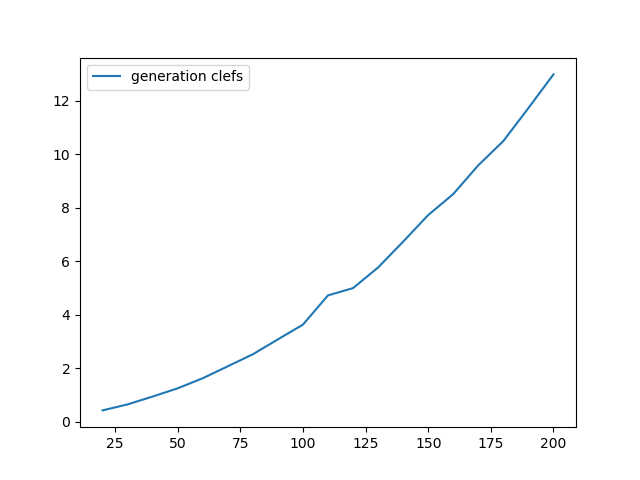
\includegraphics[scale=0.49]{images/generationClef.png} 
    \end{center}
\end{frame}{}

\begin{frame}{État de l'art}
    \begin{alertblock}{Avant la Thèse de Craig Gentry (2009)}
    Cryptographie partiellement homomorphe : OK
    \end{alertblock}
    \begin{alertblock}{Thèse de Craig Gentry (2009)}
    Astuce : bootstrap
    \end{alertblock}
\end{frame}{}


\addtocontents{toc}{\protect\setcounter{tocdepth}{2}}

%fin de l'introduction : rajouter le schéma va-et-vient  + finir l'etat de l'art